\documentclass[11pt,a4paper,fontset=none]{ctexart}

\setCJKmainfont{Songti SC}
\setCJKsansfont{PingFang SC}
\setCJKmonofont{Songti SC}

\usepackage[margin=2.15cm]{geometry}
\usepackage{amsmath,amssymb,bm}
\usepackage{booktabs,longtable,tabularx,array,multirow}
\usepackage{xcolor}
\usepackage{enumitem}
\usepackage{hyperref}
\usepackage{fancyhdr}
\usepackage{graphicx}
\usepackage{float}
\usepackage{caption}
\usepackage{microtype}
\usepackage{multicol}

\definecolor{RadarBlue}{HTML}{1F4E79}
\definecolor{RadarGreen}{HTML}{287A52}
\definecolor{RadarOrange}{HTML}{B85C20}
\definecolor{RadarRed}{HTML}{A33A32}
\definecolor{RadarGray}{HTML}{5B6573}
\definecolor{RadarLight}{HTML}{EEF3F7}

\hypersetup{
  colorlinks=true,
  linkcolor=RadarBlue,
  urlcolor=RadarBlue,
  citecolor=RadarBlue,
  pdfauthor={Radar Cube-to-Dense Project},
  pdftitle={4D Radar Cube to Dense Point Cloud: Work Report 2026-08-07}
}

\setlist[itemize]{leftmargin=1.7em,itemsep=0.22em,topsep=0.35em}
\setlist[enumerate]{leftmargin=1.9em,itemsep=0.22em,topsep=0.35em}
\renewcommand{\arraystretch}{1.18}
\setlength{\emergencystretch}{3em}
\captionsetup{font=small,labelfont=bf}

\newcommand{\done}{\textcolor{RadarGreen}{\textbf{已验证}}}
\newcommand{\impl}{\textcolor{RadarBlue}{\textbf{已实现}}}
\newcommand{\pending}{\textcolor{RadarOrange}{\textbf{待实验}}}
\newcommand{\running}{\textcolor{RadarOrange}{\textbf{运行中}}}
\newcommand{\closed}{\textcolor{RadarRed}{\textbf{未通过}}}
\newcommand{\locked}{\textcolor{RadarGray}{\textbf{锁定}}}
\newcommand{\code}[1]{\texttt{#1}}
\newcommand{\hash}[2]{{\small\ttfamily #1\allowbreak{}#2}}
\newcommand{\metric}[1]{\textbf{#1}}
\newcommand{\raed}{\mathrm{RAED}}
\newcommand{\xyz}{\mathrm{XYZ}}
\newcolumntype{Y}{>{\raggedright\arraybackslash}X}

\pagestyle{fancy}
\fancyhf{}
\fancyhead[L]{4D Radar Cube-to-Dense}
\fancyhead[R]{工作报告 2026-08-07}
\fancyfoot[C]{\thepage}
\setlength{\headheight}{14pt}

\title{\bfseries 从 4D Radar Cube 生成物理一致的稠密点云\\[0.45em]
\large 当前网络、证据审计与几何输出契约修订}
\author{Radar Cube-to-Dense 项目组}
\date{2026 年 8 月 7 日}

\begin{document}
\maketitle

\begin{center}
\fcolorbox{RadarBlue}{RadarLight}{
\begin{minipage}{0.92\textwidth}
\small
\textbf{报告口径。}
本文只采用当前仓库中的冻结协议、H200 结果文件、运行日志和代码实现形成科研结论；
尚未归档的服务器进度只作为运行观察。状态截点为
\textbf{2026-08-07 本次归档完成时}。文中严格区分“已实现”“已验证”、
“已跳过”和“仅计划”：
结构 oracle、验证集 GT 排序和单帧 memorization 不能替代可部署模型结果；
旧 TruckScenes 点云时序实验只能支持机制动机，不能验证当前 K-Radar Cube 主线。
截至截点，数据审计 G0 已通过；R-B2 当前 Cube-only 激活家族已按完整
76 帧审计关闭；Q1-R 的同源重放、full-24 诊断与证书也已完成。
重放没有通过预注册的原模型端点等价门，因此旧 Q1-R 八帧 quality training
在启动前跳过。
原 R-A1 checkpoint 文件已在存储清理中删除；新 checkpoint 只能称为
\textbf{同源同协议重放}，不得称为原 checkpoint 的同一复现。
在此边界上，项目已另行冻结新命名的 \textbf{Q-Local-F0}：它只把
Fresh-WCE-20 当作新鲜候选场，保持 700k 坐标与 exact-10k exporter 不变，
学习由局部 Full-RAED 证据决定的六档几何风险分布。其 source-bound H200
预检已以 \code{qlocal\_f0\_capacity\_no\_go} 原子终止：10/12 帧的不可部署
oracle 通过，但两个 fit 帧失败，因此 scorer 训练未启动。失败同时暴露了逐帧
固定 $8000/1700/300$ 距离配额可能与 $0.8$ m Chamfer/5\% outlier 门矛盾；76-frame train-only
配额可行性审计已冻结。逐点 Doppler、Cube-cycle、时序生成和测试集评估仍未解锁。
\end{minipage}}
\end{center}

\tableofcontents
\newpage

\section{执行摘要}

\subsection{项目要解决的问题}

项目的最终目标是从当前帧完整 4D Radar Cube
\begin{equation}
  \mathbf C_t\in\mathbb R_{\ge 0}^{D\times R\times A\times E},
  \qquad (D,R,A,E)=(64,256,107,37),
\end{equation}
生成固定数量、雷达可观测的稠密状态
\begin{equation}
  \mathcal P_t=
  \left\{\mathbf p_i=(x_i,y_i,z_i),\;
  q_i(v_r),\;c_i\right\}_{i=1}^{10{,}000}.
\end{equation}
其中 $q_i(v_r)$ 是逐点环形 Doppler 分布，$c_i$ 是可观测置信度。
后续再将历史状态经 ego motion 与 Doppler/flow 传播为先验，由当前 Cube
重新决定当前时刻的几何、速度和置信度。

该问题区别于普通“单帧稀疏点云超分辨率”：输入不是 CFAR 后的稀疏点，
输出也不仅是更密的 XYZ。目标是联合生成
\textbf{位置、速度分布和置信度}，并用 point-to-Cube 重投影与跨帧运动关系
约束物理一致性。

\begin{figure}[H]
  \centering
  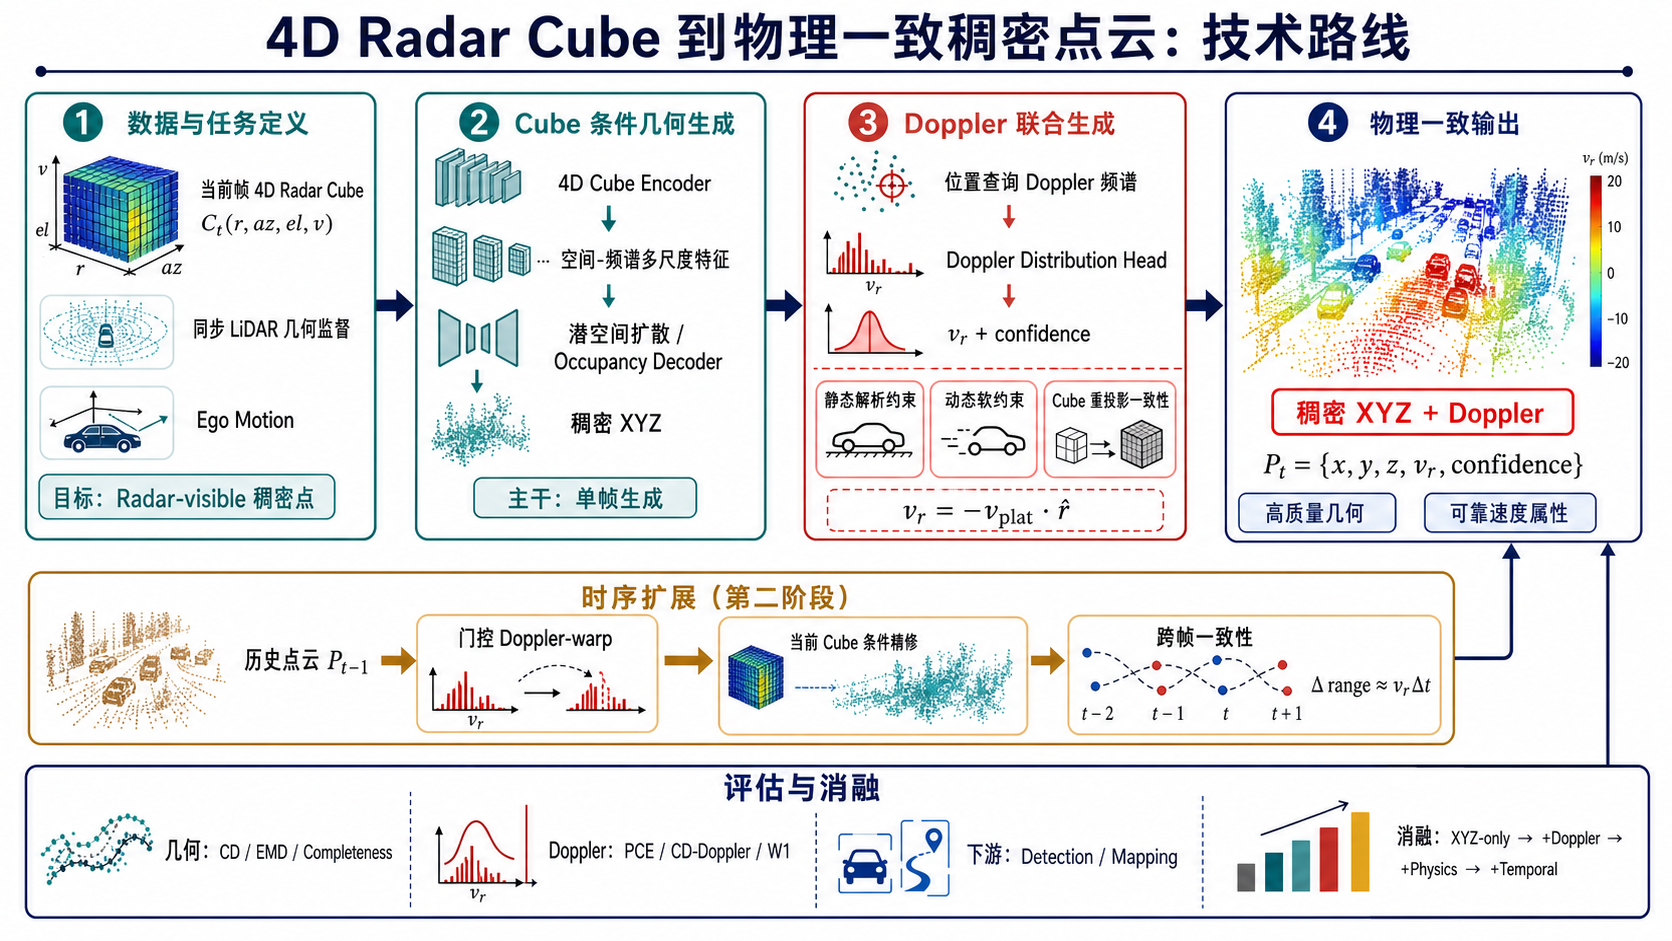
\includegraphics[width=\textwidth]{../docs/assets/cube_to_dense_technical_roadmap.png}
  \caption{目标系统技术路线。当前已验证的是数据协议与单帧几何诊断；
  图中的 Doppler 联合生成、Cube 重投影闭环和时序扩展仍受几何父模型门控，
  本图不表示这些下游模块已经通过实验。}
  \label{fig:roadmap}
\end{figure}

\subsection{当前最重要的结论}

\begin{enumerate}
  \item \textbf{数据链已可信。}
  修复版 G0 覆盖 45 个场景、100 帧，76/24 train/validation 分区保持场景隔离，
  100/100 帧成功且 11/11 项检查通过。

  \item \textbf{RAE-Max 出现几何指标正信号，但未通过几何父模型门。}
  RAE-Max 将 CFAR 的 Chamfer 从 $10.6982$ m 降至 $2.9306$ m，
  但 $25.697\%$ 的离群率高于冻结的 $25\%$ 门，且远距 completeness
  没有形成全面优势，因此不能表述为方法通过。
  Full-RAED 的 Chamfer 为 $3.1024$ m，相对 RAE-Max 恶化 $5.86\%$，
  场景优先 95\% 区间为 $+0.78\%$ 到 $+14.69\%$。

  \item \textbf{RaLD 原生解码不直接满足 fixed-10k contract。}
  G1D、G1G、R-A1 和 R-A2 均完成各自冻结实验但未通过几何门。
  官方 RaLD 原生采用变长 occupancy threshold，而本项目要求固定 10k、
  三段距离配额和 5 cm 最小间距；本项目已测试的 RaLD-inspired fixed-count
  adaptations 尚未通过。把 binary occupancy confidence
  直接当成几何质量分数，是本项目额外引入且已被实验证伪的假设。

  \item \textbf{核心瓶颈已经从“有没有候选”定位到“如何评分和结构化输出”。}
  历史 R-A1 checkpoint 的 700k 固定候选对 GT 的 target-to-candidate 平均距离为
  $0.1486$ m。仅用验证集 GT 重新排序、保持候选和 exact-10k 导出不变，
  Chamfer 可从 $4.0090$ m 降到 $0.6410$ m，离群率从 $31.8129\%$
  降到 $2.2804\%$。这不是可部署结果，但证明候选支撑充足，主要失败位于
  confidence-quality alignment。新的 replay pool 已在 full-24 diagnosis 中
  独立复现同一机制分支：current-confidence 的 $4.0261$ m/$31.7854\%$
  Chamfer/离群率，经不可部署 GT 排序变为 $0.6375$ m/$2.2771\%$。

  \item \textbf{R-B2 当前激活家族已被完整审计关闭。}
  80k \code{max\_d} arm 的 occupied-voxel recall 在 76/76 训练帧均过
  20\% 门，但 3 帧 confidence coverage 低于 30\%，最低仅 14.6397\%。
  因此不启动 memorization 或正式训练；该结论不否定 voxel-slot 的
  GT-aided 表示容量，只关闭 score-plus-fixed-neighborhood 激活机制。

  \item \textbf{Q1-R 在父模型授权门停止，quality 假设本身尚未被训练检验。}
  source \code{f2a9489} 的 20-epoch replay 已在物理 H200 GPU2 完成。
  source/data/runtime、固定 Q0、replay-specific Q1、full-24 GT 排序诊断和
  禁止访问检查全部通过；但 replay 相对归档端点的 median completeness、
  far completeness、condition effect 和 matched-win 四项差异超过冻结容差。
  证书状态为 \code{replay\_parent\_not\_authorized\_for\_q1r\_tiny}，
  因此八帧训练与条件式 Q2 均未启动，不能把它们写成方法失败。

  \item \textbf{Q-Local-F0 已在容量门停止，不能训练。}
  Fresh-WCE-20 的 700k 候选、Q0/Q1、residual、parent confidence 与 exporter
  全部冻结；新 scorer 从归一化 RAE、冻结全局 condition latents、局部完整
  64-bin Doppler spectrum、能量、谱熵和 R/A/E 梯度预测六档最近表面距离分布，
  以负期望距离排序。该路线不继承已失败的 Q1-R 父认证，也不再训练 binary
  occupancy；它是一个新命名、train-only、可独立证伪的几何分支。真实预检中
  10/12 帧通过，但 $(47,514)$ 的 CD/outlier 为 $1.4250$ m/$7.0\%$，
  $(58,404)$ 为 $2.2598$ m/$20.0\%$，超过逐帧 $0.8$ m/$5\%$ 门。

  \item \textbf{Q-Local 的工程机制通过，但不能覆盖容量 no-go。}
  8 个 fit 序列帧与 4 个 unseen-train 序列帧全部来自 76-frame train split；
  wrong-Cube arm 只交换全局/局部 Cube 证据，候选坐标、parent confidence、
  target 和 exporter 保持相同。训练上限为 500 updates 或 7200 GPU-seconds；
  模型共 380,818 个参数；六组梯度均有限且非零，同坐标 intervention 保持
  candidate hash 相同并改变 local spectrum/global condition/score，所有 12 帧
  exact-count、配额、唯一性和真 5 cm 结构检查均通过。尽管如此，每帧
  GT-nearest capacity oracle 的 $\mathrm{CD}\le0.8$ m、outlier $\le5\%$ 是前置
  硬门；两个 fit 帧失败后，500-update 训练被正确禁止。

  \item \textbf{失败进一步指向输出契约，而不只是候选场。}
  $(58,404)$ 的 target 全部位于 30 m 内，而 exporter 强制输出 1,700 个
  30--60 m 点和 300 个 60--120 m 点；其 oracle outlier 恰为 20\%。这提示
  固定逐帧 range quota 可能给出与模型无关的矛盾下界。当前先对全部
  76 个 train 帧做 reverse-triangle-inequality 审计；若任一帧的乐观 Chamfer
  下界超过 $0.8$ m 或强制 outlier 超过 5\%，任何后继 exporter 均不得继承旧配额。

  \item \textbf{文献重扫后，创新边界进一步收紧。}
  RaUF、SDDiff、RadarMP、Radar-Mamba 与 DoppDrive 已分别覆盖雷达不确定性、
  spatial--Doppler 建模、连续 tesseract、历史增强或 Doppler 时序传播。
  因而不能主张“首次使用 Doppler 墠密”或“首次多帧雷达增强”。最终可防守目标是
  exact-count XYZ、逐点环形 Doppler 分布和 calibrated confidence 的联合状态，
  再同时满足 point-to-RAED closure 与 displacement--Doppler consistency。
\end{enumerate}

\subsection{状态总表}

\begin{table}[H]
\centering
\small
\caption{截至 2026-08-07 的阶段状态}
\begin{tabularx}{\textwidth}{>{\bfseries}p{2.2cm} p{2.3cm} Y Y}
\toprule
阶段/路线 & 状态 & 已取得的证据 & 当前边界 \\
\midrule
G0 数据审计 & \done & 100/100 帧，11/11 检查通过 & 只证明数据、坐标、同步和 target 构造可信 \\
原 G1 Cube U-Net & \closed & RAE-Max 明显优于 CFAR & Full-RAED 未优于 RAE-Max，且绝对离群门失败 \\
G1D RaLD query field & \closed & 150 epochs 与 D1--D3 诊断完成 & 条件使用弱、重复和 coverage/precision 矛盾未解决 \\
G1G condition-exclusive & \closed & 信息路径和梯度检查通过 & condition shuffle、离群和重复门失败 \\
R-A1 RaLD-WCE & \closed & 学到显著 Cube 条件效应；700k pool 支撑强 & binary confidence 无法可靠选择 exact-10k \\
R-A2 binary pilot & \closed & 8 帧、500 updates 完成 & memorization 仍未通过，旧 sampler 同时不合格 \\
Q1-R quality ranking & \closed & replay、full-24 diagnosis 与证书完成；ranking bottleneck 再现 & replay 端点等价门失败，tiny 与 Q2 未启动 \\
Q-Local-F0 & \closed & 10/12 oracle 帧通过；梯度、同坐标干预、结构与 provenance 通过 & 两个 fit 帧容量失败；训练按协议禁止，不代表 scorer 学习失败 \\
固定 range quota 审计 & \running & 已冻结严格径向 Chamfer/outlier 下界与 76-frame train-only 协议 & 正在执行；决定后继 exporter 是否必须取消硬配额 \\
R-B2 voxel-slot & \closed & GT-aided 结构容量通过；80k arm 的 recall 在 76/76 帧过门 & 3 帧 coverage 失败，当前 Cube-only activation family 关闭 \\
G4 时序数据 & \running & 45 序列、2,160 帧、约 600.8 GiB 已下载 & exact-member/size/CRC 审计运行中；不解锁时序训练 \\
下游物理与时序 & \locked & 代码和旧机制证据存在 & 无通过的 K-Radar 几何父模型，不能形成当前主张 \\
\bottomrule
\end{tabularx}
\end{table}

\section{研究定位与创新边界}

\subsection{与传统雷达点云增强的关系}

传统雷达增强通常把任务写成单帧稀疏点或单帧 BEV 的去噪、补全或超分辨率。
本项目的更准确定位是：
\begin{quote}
\textbf{传统方法把雷达增强看成单帧几何稠密化；本项目把它定义为完整
RAED 测量条件下的雷达状态生成问题。}模型不仅输出当前位置，还应输出
与该位置匹配的 Doppler 分布和置信度，并在后续阶段用历史状态改善连续性，
同时接受当前 Cube 的观测纠正。
\end{quote}

“使用历史帧”本身不能作为创新。Radar-Mamba、RadarMP、DoppDrive、
RMap、CMFlow 等已经覆盖多帧增强、scene flow 或历史聚合。
可防守的差异应同时满足以下四点：
\begin{itemize}
  \item 当前完整 Cube 始终是主观测，而不是只从上一帧自回归；
  \item 输出是新生成的固定计数雷达状态，而不是历史测量点的直接累加；
  \item Doppler 是逐点生成属性或分布，而不是只作为输入 feature；
  \item 生成状态必须同时满足 Cube 重投影与跨帧位移--速度一致性。
\end{itemize}

\subsection{当前可主张与不可主张内容}

\begin{table}[H]
\centering
\small
\caption{创新主张的证据边界}
\begin{tabularx}{\textwidth}{>{\bfseries}p{4.0cm} p{2.2cm} Y}
\toprule
主张 & 当前状态 & 准确表述 \\
\midrule
完整 RAED 条件可直接改善几何 & 否决 & 早融合 Full-RAED 在当前协议下未优于 RAE-Max \\
RaLD 风格 wide query 提供足够支撑 & 诊断支持 & 700k pool 覆盖强，但 learned exact-10k selector 未通过 \\
局部 Full-RAED 风险评分可替代 binary occupancy & 未评估 & Q-Local scorer 已实现，但父候选/配额 capacity gate 先失败，模型未训练 \\
voxel-slot 能表达固定 10k & 结构支持/激活失败 & GT-aided oracle 通过；当前 Cube-only 激活家族在 76 帧 support gate 失败 \\
生成逐点 Doppler 分布 & 仅计划 & 代码存在，但 geometry parent 未过门，不能评价 \\
Cube-point 双向物理闭环 & 仅计划 & renderer 与损失存在，尚无有效父模型上的消融 \\
历史 Doppler/flow 改善长期一致性 & 仅机制证据 & 旧点云管线有证据；K-Radar Cube 主线尚未验证 \\
\bottomrule
\end{tabularx}
\end{table}

\section{数据、计算与评估协议}

\subsection{数据与输入}

K-Radar Cube 从磁盘布局 $(D,R,E,A)$ 转为规范
$(D,R,A,E)=(64,256,107,37)$。每帧保留完整 64-bin Doppler 轴。
开发 cohort 共 100 帧、45 个场景，按场景划分为 76 个训练帧和
24 个验证帧；测试集在模型族冻结前保持不可访问。

监督目标不是完整 LiDAR，而是经过雷达视场、Cube 支撑和配准约束构造的
radar-observable dense target。每个目标点保存 XYZ、可观测置信度和
RAE 映射。修复版 G0 的关键检查包括：
\begin{itemize}
  \item Cube shape、数值有限性、轴单调性与 CFAR exact-bin round trip；
  \item LiDAR/雷达时间同步与 odometry 支撑；
  \item 方位正负号与镜像对照；
  \item target nonempty、跨帧 observability 稳定性；
  \item train-only 时间参考选择与 no-deskew 冻结。
\end{itemize}

\subsection{输出与硬约束}

正式几何输出固定为 10,000 点，并要求：
\begin{equation}
  N_{0-30}=8{,}000,\qquad
  N_{30-60}=1{,}700,\qquad
  N_{60-120}=300.
\end{equation}
点间真实欧氏距离不得小于 5 cm；禁止通过复制、padding、重复中心或
后处理 jitter 伪造点数。评估至少报告：
\begin{itemize}
  \item 对称 Chamfer、confidence-weighted completeness、F-score；
  \item 2 m 离群率、5 cm 重复率与 exact-count；
  \item 0--30、30--60、60--120 m 分层指标；
  \item wrong-condition 干预和 matched-condition win rate；
  \item 后续 Doppler 的 circular W1/NLL/PCE、Cube spectrum discrepancy；
  \item 后续时序的 radial consistency、flicker 与多步 rollout。
\end{itemize}

\subsection{计算与可复现边界}

所有科研计算限定在 \code{wangning} 用户的 NVIDIA H200 节点，
只允许物理 GPU 0 或 2；物理 GPU 1 的 RTX 5000 不使用。
Conda 环境为
\code{/home/wangning/miniforge3/envs/hym\_radar}。
原 R-A1 运行只绑定 source、manifest、split、normalization 与 evaluator；
Q1-R 及后续正式运行才强制进一步绑定 cache、逐 Cube、资源文件、checkpoint、
metrics、diagnosis 和 evaluator 的 SHA-256。两种 provenance 强度不能混称。

当前本地分支为 \code{agent/cube-to-dense-g0}。Q1-R 终局证书所绑定的
审计实现初次证书提交为
\hash{137e766f5d13acd38a5f0296d93bb821}{df6c15fe}；恢复事务与逐帧证据链
二次加固提交为
\hash{e159a22c5343e81c0cf29351da07290a}{686edba5}。
R-B2 support sweep 已以 source \code{fec8f81} 归档并推送；初版 Q1 以
\code{252fa7b} 推送；Q1-R 的 replay-parent certificate、provenance hardening
初版由 \code{60be31d} 提交并完成 102 项 H200 相邻回归；二次独立审计修正由
\code{137e766} 形成首轮证书；二次审计后由 \code{e159a22} 实现终态恢复、
逐帧重聚合、current-confidence hash/geometry control 与主路径 staging，
并在新的干净 H200 快照完成 42 项定向与 101 项扩大回归。
真实归档 formal metrics 也已逐帧重算并与落盘 decision 完全一致。
证书后的独立静态终审另发现 3 项 P1 和 3 项 P2，因此
\code{e159a22} 只作为本次 no-go 的实现与证据来源，不是可复用的训练授权基线。

新路线 Q-Local-F0 的冻结与预检实现提交为
\hash{bf1a166c48be60f82c5283b5937edf0c}{f6ad64c2}。它逐项关闭上述终审边界：
从原始 Cube/cache 重建 non-deployable capacity oracle；强制 12 帧身份、顺序和
wrong-Cube 配对；terminal 采用 staging 后原子提交；记录物理 GPU index、UUID、
PCI bus ID 与 visible-device map；并增加 drop、duplicate、partition tamper、
原子失败报告和 GPU parser 等对抗性测试。干净 H200 快照已经通过
52 项 Q-Local/Q1 定向测试与 522 项完整回归。真实 12-frame preflight 在物理
H200 GPU2 上用时 444.58 s，峰值 allocated memory 为 2.432 GB，并原子落盘
\code{qlocal\_f0\_capacity\_no\_go}。完整 provenance、gradient 与 intervention
检查均通过；训练未启动。

\section{模型结构与路线演化}

\subsection{当前网络总览}

当前代码库不是一个已经端到端通过的单体网络，而是由冻结上游、候选生成、
排序导出和受门控下游组成的模块链。表~\ref{tab:network-overview} 区分了
结构资产与可用科学结果。

\begin{table}[H]
\centering
\small
\caption{当前神经网络与模块状态}
\label{tab:network-overview}
\begin{tabularx}{\textwidth}{>{\raggedright\arraybackslash\bfseries}p{2.5cm} >{\raggedright\arraybackslash}p{3.8cm} Y >{\raggedright\arraybackslash}p{2.0cm}}
\toprule
模块 & 输入/核心结构 & 输出与作用 & 状态 \\
\midrule
Cube U-Net & RAE-Max、RAE-Moments 或 64-bin Full-RAED；3D residual U-Net & RAE occupancy/residual；建立最小单帧几何基线 & 已训练，未过正式门 \\
G1D query field & 336 radar tokens、512 working latents、24 个 conditioned blocks、coarse-to-refine queries & arbitrary-query occupancy 与 residual & 已训练并关闭 \\
R-A1 RaLD-WCE & 500k Q0 + 200k Cube-guided Q1；condition-exclusive field & 700k frozen candidates，随后 exact-10k capacity export & 已训练并关闭；保留历史诊断与生成机制，不保留原 pool 字节身份 \\
Q1-R quality head & refined RAE、512-d frozen condition latents、detached occupancy confidence；Fourier embedding + 4-head cross-attention + MLP & 每候选连续 quality correction，只替换排序分数 & 已实现；父证书 no-go，训练未启动 \\
Q-Local-F0 & normalized RAE、detached parent confidence、冻结全局 latents、局部 64-bin spectrum、能量/熵/梯度；cross-attention + 6-bin risk head & 最近表面距离分布及负期望风险排序；坐标与 exporter 不变 & 已实现；capacity no-go，训练未启动 \\
R-B2 voxel-slot & 0.4 m Cartesian voxels、每 voxel 4 slots & whole-voxel fixed-count export & 容量 oracle 通过，激活家族关闭 \\
Doppler 与 Cycle & final-position Cube spectrum query、64-bin distribution head、differentiable splatting & $q_i(v_r)$、confidence 与 Cube closure & 已实现，未解锁 \\
Temporal & ego/Doppler warp、token/latent/query fusion、scheduled sampling & 当前 Cube 校正的时序状态与 rollout & 已实现，未解锁 \\
\bottomrule
\end{tabularx}
\end{table}

Q1-R 的预注册候选数据流可写为
\begin{equation}
\mathbf C_t
\xrightarrow{\text{frozen RaLD-WCE}}
\{\widetilde{\mathbf u}_i,p_i^{\mathrm{occ}},\mathbf Z_C\}_{i=1}^{700k}
\xrightarrow{\text{Q1-R quality head}}
\{s_i^Q\}_{i=1}^{700k}
\xrightarrow[5\,\mathrm{cm}]{8000/1700/300}
\widehat{\mathcal P}_t^{10k}.
\end{equation}
若训练获授权，GT 只会在完整 700k candidates 构造后生成 soft quality target；
推理 API 不接受 GT。当前 replay-parent 证书 no-go，因此该 quality head 没有进入
梯度更新，公式描述的是实现和冻结协议，不是已有训练结果。

Q-Local-F0 与旧 Q1-R 的关键差异是：它不再要求 Fresh-WCE-20 与已删除 checkpoint
端点等价，也不把 geometry target 压缩为单个 soft occupancy correction。它把
fresh replay 明确降级为冻结候选生成器，并用当前 Cube 的局部测量证据估计几何风险。

\subsection{基础 Cube U-Net}

\code{CubeOccupancyNet} 在 RAE 网格上使用轻量 3D residual U-Net。
三种 matched 输入编码分别为：
\begin{itemize}
  \item \textbf{RAE-Max：}沿 Doppler 维取最大强度；
  \item \textbf{RAE-Moments：}峰值、Doppler 均值和标准差；
  \item \textbf{Full-RAED：}将 64 个 Doppler bins 作为输入通道。
\end{itemize}
三者先投影到相同 base width，再进入两层下采样与 skip-connected 上采样。
occupancy head 输出 RAE 网格 logits，早期版本直接选取全局 top-10k cell
center。该结构证明稠密解码本身显著强于 CFAR，但也暴露 binary occupancy
在固定计数尾部的离群问题。

\subsection{RaLD query-field 路线}

G1D 按 RaLD 思路构建 512 个 working latents、24 个 radar-conditioned
Transformer blocks、32k coarse proposals 与 10k local refinement points。
训练查询遵循约 6.25\% occupied 与 93.75\% empty 的 classwise occupancy
监督，推理则使用 radar-guided coarse-to-refine queries。

这一实现比早期 deterministic latent refiner 更接近 RaLD 的 query-field
结构，但仍与官方方法存在重要差异：官方 RaLD 的生成结果是对任意 query
做 occupancy threshold 得到的变长集合；当前项目必须在范围配额和间距约束下
输出精确 10k。因此，G1D 的失败不能解释为“没有借鉴 RaLD”，也不能把
RaLD 的公开结果直接当作当前任务的 baseline 结果。

\subsection{R-A1：Wide Candidate Export}

R-A1 将训练与导出拆成两个层次：
\begin{enumerate}
  \item Q0 在全空间构造 500k 规则 queries；
  \item Q1 围绕 Cube peaks 构造 200k radar-guided queries；
  \item 冻结 field 对 700k 候选预测 occupancy 和 residual；
  \item 在三段距离配额与 5 cm capacity-one 约束下导出 exact-10k。
\end{enumerate}
该路线学到了可测量的 current-Cube condition effect，但最终 confidence
仍混合了“是否占据”和“几何定位是否精确”两个不同问题。

\subsection{Q1-R：连续几何质量头与重放父模型认证}

Q1-R 的设计要求相对通过认证的 replay parent 保持 field、Q0/Q1 机制、该 parent 的候选坐标、
residual、范围配额和导出约束不变，只新增独立质量头。它不声称 replay pool 与
已删除 checkpoint 的历史 pool 字节相同。输入为：
\begin{equation}
  \left(\widetilde{\mathbf u}_i,\;\mathbf Z_C,\;
  \operatorname{stopgrad}(p_i^{\mathrm{occ}})\right),
\end{equation}
其中 $\widetilde{\mathbf u}_i$ 是候选的归一化连续 RAE 坐标，
$\mathbf Z_C$ 是冻结的当前 Cube condition latents。
质量头使用 Fourier coordinate embedding、condition cross-attention
与 MLP residual：
\begin{equation}
  s_i^{Q}
  =\operatorname{logit}(p_i^{\mathrm{occ}})+\Delta s_i.
\end{equation}
最后一层零初始化，因此 update 0 必须与 R-A1 的排序和 selected rows
bit-exact 一致。

训练目标由当前帧 GT 仅在候选生成完成后构造：
\begin{equation}
  q_i=
  \frac{w_{j(i)}}{\max_j w_j}
  \exp\left(-\frac{\lVert\mathbf p_i-\mathbf y_{j(i)}\rVert_2}{1\,\mathrm m}\right),
\end{equation}
损失为三段距离平衡的 soft BCE 加 within-range pairwise ranking。
正式 field 全冻结，Q1-R 推理 API 不接受 GT、future、test、Doppler target
或 best-of-$k$ 输入。

原 formal R-A1 checkpoint 已在归档中记录 SHA-256：
\begin{center}
  \small\ttfamily
  5be30e0f1ca23ea3b603abb0f5e330efd3599167362a8e23ab3a5967c411a2a0
\end{center}
但对应文件已在共享存储清理中删除，无法恢复原字节。Q1-R 因此新增
source-bound replay certificate，要求 source、seed、config、输入哈希与
epoch-20 endpoint decision 一致，并重新运行 24 帧 failure-factor diagnosis。
固定 Q0 查询必须与归档逐帧一致；learned occupancy-dependent Q1 允许随 replay
checkpoint 改变，但必须由 replay-bound diagnosis 对 replay metrics 逐帧复现。
证书必须显式记录 replay checkpoint 是否与原 SHA 相同；若不同，只能称为
\textbf{source/config/data-equivalent replay parent}，不能称为 original parent。

两轮独立审计要求 Q1-R 在训练前完成以下修复，当前实现均已覆盖：
\begin{itemize}
  \item 强制调用 formal 24-frame metrics validator，并要求 epoch 20；
  \item 将八帧 Cube、\code{info\_arr.mat} 与 \code{arr\_doppler.mat}
  从“只记录哈希”升级为 expected-hash 硬门；
  \item uniform 半样本严格排除完整 top-10\% quality pool；
  \item numeric gate 与 matched/wrong exact-10k、真 5 cm 结构门共同决定通过；
  \item 每次评估保存不可覆盖的 \code{checkpoint\_updateXXXX.pt}；
  \item 证书绑定 replay checkpoint、metrics、manifest 与 full-24 diagnosis。
  \item certifier 从逐帧 formal/diagnosis 报告重算 aggregate 与 decision，trainer
  再独立调用 certifier，拒绝外部伪造的 all-true 文档；
  \item archived/replay/diagnosis 必须同为 H200 且 Torch 版本一致；
  \item candidate preparation 纳入 resume contract，评估 checkpoint/metrics
  支持中断后的不可变重放。
\end{itemize}

\subsection{Q-Local-F0：局部 Full-RAED 分布式几何风险}

Q-Local-F0 是 Q1-R no-go 之后重新冻结的独立路线。父场统一称为
\textbf{Fresh-WCE-20}，其 checkpoint SHA-256 为
\hash{c0ebb4c1509c3d36b6834bd39977cb1c}{da2fcaff1747eabc97ebb41af0f06ce4}。
该名称只表示一个新鲜候选生成器，不表示与已删除 R-A1 checkpoint 字节相同，
也不继承失败的 replay-parent authorization。

对候选 $i$，模型读取
\begin{equation}
  \mathbf h_i = \bigl[
    \phi(\widetilde{\mathbf u}_i),
    \operatorname{stopgrad}(\ell_i^{\mathrm{occ}}),
    \mathbf z_C,
    \widetilde{\mathbf s}_i^{64},
    e_i,\;H_i,\;\nabla_{R,A,E} e_i
  \bigr],
\end{equation}
其中 $\widetilde{\mathbf s}_i^{64}$ 是在 refined candidate 位置查询并归一化的
完整 Doppler log-power spectrum，$e_i$、$H_i$ 和 $\nabla e_i$ 分别表示标准化
积分能量、谱熵与 R/A/E 能量梯度。coordinate/local token 通过 cross-attention
读取冻结全局 condition latents，六分类头输出
\begin{equation}
  \boldsymbol\pi_i=\operatorname{softmax}(f_\theta(\mathbf h_i)),\qquad
  \mathbf b=(0.05,0.175,0.375,0.75,1.5,3.0)\ \mathrm m,
\end{equation}
并以负期望风险
\begin{equation}
  s_i^{\mathrm{deploy}}=-\sum_{k=1}^{6}\pi_{ik}b_k
\end{equation}
送入完全不变的 exact-10k exporter。模型参数不超过 2M；Fresh-WCE field、
候选坐标、base confidence、Q0/Q1 和 residual 全部冻结。

监督距离 $d_i$ 只在 target-free 700k candidate/evidence field 已构造后计算，
并 stop-gradient 地线性分配到相邻距离档。冻结损失为
\begin{equation}
  \mathcal L = \operatorname{mean}_{r\in\{0\!:\!30,30\!:\!60,60\!:\!120\}}
  \mathcal L_{\mathrm{dist}}^{(r)}
  +0.5\operatorname{mean}_{r}\mathcal L_{\mathrm{list}}^{(r)}.
\end{equation}
每次更新确定性采样 16,000 个互异候选，按 $12800/2720/480$ 保持三段距离配额。
推理 API 不允许 target、future/test record、selection index、随机 sample ID
或 best-of-$k$ 参数。

\paragraph{冻结 cohort 与反事实。}
fit 帧为 $(1,232),(9,440),(21,402),(27,403),(29,399),(35,403),(47,514),(58,404)$；
unseen-train 帧为 $(5,429),(26,403),(42,408),(50,405)$。两组分别按固定环映射
构造 wrong Cube。wrong arm 只重算 $\mathbf z_C$ 与局部 spectrum/energy/gradient；
Q0/Q1 rows、candidate XYZ、parent confidence、target 和 exporter 均保持 bit-identical。
因此几何变化不能由换坐标伪装为 condition dependence。

\paragraph{预检与训练门。}
训练前从原始 Cube 和 cache 独立重建全部 12 帧。不可部署的 GT-nearest
capacity oracle 必须在每帧同时满足
\begin{equation}
  \mathrm{CD}\le0.8\ \mathrm m,\quad
  \mathrm{Outlier}_{2m}\le5\%,\quad
  N=10{,}000,\quad N_r=(8000,1700,300),\quad d_{\min}\ge0.05\ \mathrm m.
\end{equation}
预检还要求两步反向传播覆盖所有 scorer 参数组、同坐标 wrong-Cube 证据有效、
输入/源代码/GPU provenance 完整且终态原子落盘。只有全部通过才允许最多 500
updates/7200 GPU-seconds 的 tiny run。连续两个 evaluation 的 fit 均满足
$\mathrm{CD}\le1.0$ m、completeness $\le0.75$ m、outlier $\le10\%$，且后一个
checkpoint 在四个 unseen-train 帧达到至少 30\% Chamfer 改善、5 pp outlier
改善、3/4 matched 胜 wrong、wrong mean Chamfer 恶化至少 5\%，才可晋级 76/24
正式几何实验。该门本身不解锁 Doppler、cycle、temporal 或 test。

\paragraph{实际预检结果。}
source \code{bf1a166} 在物理 H200 GPU2 上完成 12 帧重建并原子终止为
\code{qlocal\_f0\_capacity\_no\_go}。10 帧通过全部 oracle 门，两个 fit 帧失败：
\begin{table}[H]
\centering
\small
\caption{Q-Local-F0 失败帧的 non-deployable GT-nearest capacity oracle}
\begin{tabular}{lrrrrrl}
\toprule
帧 & target 数 & CD (m) & Completeness (m) & Outlier & $d_{\min}$ (m) & 结构门 \\
\midrule
47:514 & 1,404 & 1.4250 & 0.0878 & 7.0\% & 0.050004 & 全部通过 \\
58:404 & 285 & 2.2598 & 0.1057 & 20.0\% & 0.050008 & 全部通过 \\
\bottomrule
\end{tabular}
\end{table}
所有 12 帧均保持 700k candidates、exact 10,000、$8000/1700/300$、unique rows、
无 copy/padding/jitter 和真 5 cm spacing。380,818 参数 scorer 的六组梯度均有限
非零；same-coordinate wrong-Cube 保持 candidate coordinate hash bit-identical，
同时改变 local spectrum、global condition 与 selection score。Fresh-WCE state
前后 hash 一致，validation/test/future 均未访问。因此这是有效的容量 no-go，
不是实现无效；由于 scorer 没有接受训练，不能把它写成 learned ranking no-go。

进一步检查表明，58:404 的 285 个 target 范围最大值为 27.877 m，而固定 exporter
强制 2,000 个点位于 30--120 m。由
$\lVert\mathbf x-\mathbf y\rVert_2\ge
|\lVert\mathbf x\rVert_2-\lVert\mathbf y\rVert_2|$，这些点不可能进入 2 m target
邻域，故至少 20\% outlier 与网络无关。该现象触发独立的 76-frame fixed-quota
feasibility audit。进一步把三个区间的最小径向 gap 按 quota 加权，并把
completeness 乐观地置零，仍得到约 $1.3245$ m 的 Chamfer 下界，同样超过
$0.8$ m 门；在审计完成前，不实现沿用相同配额的后继模型。

\subsection{R-B2：Cartesian Voxel-Slot}

R-B2 不再从 700k points 中直接做全局 hard top-$k$，而是把输出写成
固定 Cartesian voxel 与局部 slots：
\begin{itemize}
  \item voxel size 为 $0.40\times0.40\times0.40$ m；
  \item 每个 voxel 固定 4 个 XY quadrant anchors；
  \item 网络预测 voxel occupancy、4 个 slot confidence 和 4 个局部 XYZ offsets；
  \item 选择 $2000/425/75$ 个 whole voxels，每个输出 4 点；
  \item 参数化本身保证最小点距下界不小于 0.06 m。
\end{itemize}

结构 oracle 已证明这一表示在 100 帧上具备 exact-10k 容量，但第一版
Cube-only 激活只覆盖 10.976\% 的 target-occupied voxels，低于 20\% 门。
随后完成的 bounded sweep 比较三种 Cube Doppler 聚合
\code{max\_d/sum\_d/log\_sum\_d} 与 20k/40k/80k candidate banks；
任何 GT 均只在候选生成后用于 support 报告。

最强的 80k \code{max\_d} arm 将 occupied-voxel recall 修复到 76/76 帧
均不低于 20\%，但仍有 3 帧 confidence coverage 低于 30\%。因此当前
score-plus-fixed-neighborhood 激活家族已关闭，不启动 one-frame optimization。
这意味着 voxel-slot 目前只有\textbf{表示容量证据}，没有可部署 Cube-only
激活或学习结果。

\subsection{下游 Doppler、Cycle 与 Temporal 模块}

仓库已存在以下模块，但当前只能标记为实现资产：
\begin{itemize}
  \item \code{CubeDopplerNet}：scalar、64-bin distribution 和位置条件查询；
  \item \code{CubeCycleNet} 与 \code{point\_to\_cube.py}：
  连续 RAE offsets 与可微 RAED soft splatting；
  \item \code{CubeTemporalNet}、temporal prior 与 scheduled sampling：
  ego/Doppler warp、Concat、Cross-Attention 和 Draft Refinement；
  \item direct multi-horizon world model：0.5/1.5/2.5 s fixed-count 预测接口。
\end{itemize}

由于没有几何父模型通过，以上模块尚不能构成当前 K-Radar 方法结果。
特别是 D-MHW 的 birth radial-moment label 仅覆盖 4.487\% 的未来几何，
因此 birth Doppler 分支已关闭；未来若重启，只能让 birth points
输出 XYZ/confidence，并显式设置 \code{doppler\_valid=false}。

\section{实验结果与失败定位}

\subsection{原始单帧几何}

\begin{table}[H]
\centering
\caption{原始 G1 三种子结果}
\begin{tabular}{lrrl}
\toprule
方法 & Chamfer (m) & 2 m 离群率 & 判定 \\
\midrule
CFAR & 10.6982 & 79.909\% & 稀疏测量基线 \\
RAE-Max & 2.9306 & 25.697\% & 大幅改善，但绝对离群门失败 \\
Full-RAED residual & 3.1024 & 26.896\% & 相对 RAE-Max 恶化 5.86\% \\
\bottomrule
\end{tabular}
\end{table}

这组结果否决的是“当前早融合实现中完整 Doppler 频谱改善几何”的主张，
不是否决 Doppler 作为最终点属性、cycle 信号或时序运动信息的价值。

\subsection{RaLD 结构路线结果}

\begin{table}[H]
\centering
\small
\caption{RaLD 相关几何路线的关键终点}
\begin{tabularx}{\textwidth}{>{\bfseries}p{2.1cm} r r r Y}
\toprule
路线 & Chamfer & Completeness & 离群率 & 主要失败 \\
\midrule
G1D epoch 15 & 6.0103 m mean & 3.5637 m median & 17.8875\% & 23 个远距帧的 mean completeness 为 46.9407 m，重复 26.9721\% \\
G1D epoch 150 & 6.3969 m mean & 3.6331 m median & 24.8396\% & 继续训练恶化，D1--D3 均未授权修复 \\
G1G epoch 20 & 未作为主门单列 & 1.2086 m median & 84.6854\% & condition shuffle 为 $-0.1211\%$，重复 70.8108\% \\
R-A1 epoch 20 & 4.0090 m mean & 1.5081 m median & 31.8129\% & 条件效应强但 precision tail 与 matched wins 失败 \\
R-A2 update 500 & 5.1892 m mean & 1.8302 m mean & 45.2600\% & 8 帧 memorization 未通过 \\
\bottomrule
\end{tabularx}
\end{table}

G1D 的 condition intervention 进一步表明：固定 measured path 时，
替换全局 Cube 只使 mean Chamfer 变化 $+1.05\%$，且场景优先区间跨零。
这说明大模型虽有梯度路径，但 global condition use 弱且不稳定。
G1G 强制取消 local bypass 后仍没有形成有用的 condition-dependent allocation，
所以问题不能仅靠“禁止 bypass”解决。

\subsection{R-A1 frozen-pool 诊断}

\begin{table}[H]
\centering
\caption{同一 700k pool、同一 exact-10k 约束下的排序对照}
\begin{tabular}{lrrrr}
\toprule
排序 & Chamfer & Completeness & 2 m 离群率 & 远距 completeness \\
\midrule
模型 confidence & 4.00895 m & 1.50805 m & 31.8129\% & 11.12111 m \\
验证 GT nearest oracle & 0.64102 m & 0.14895 m & 2.2804\% & 0.70414 m \\
\bottomrule
\end{tabular}
\end{table}

该 oracle 在 24/24 验证帧和 23/23 远距帧上通过全部绝对几何检查，
但 GT 参与排序，因此不具备部署资格。它的作用是排除“wide field 没有好点”
这一解释，并将下一步压缩到 quality learning、uncertainty calibration
或结构化输出，而不是继续扩大同一 occupancy 网络。

\subsection{Cardinality 与结构表示诊断}

\begin{table}[H]
\centering
\small
\caption{固定输出数量与新表示的诊断}
\begin{tabularx}{\textwidth}{>{\bfseries}p{2.6cm} Y Y}
\toprule
诊断 & 结果 & 决策 \\
\midrule
RAE-Max 2.5k--10k & 点数减少会降低离群率，但 completeness 变差；10k Chamfer 最好 & exact-10k 不是主要失败因素 \\
R-B1 range-echo & $K=4/6$ 在两帧最多只有 6798/7939 等可用 peaks，无法满足三段配额 & 直接 peak construction 不训练 \\
R-B2 GT-aided oracle & $0.4$ m、4 slots：Chamfer 0.72268 m，median completeness 0.05963 m，outlier 1.5417\% & 结构容量通过，但不是模型结果 \\
R-B2 Cube-only 20k & exact/unique/配额均通过；occupied-voxel recall 10.9763\%，confidence coverage 31.6908\% & 第一版激活 no-go；只授权 bounded support sweep \\
R-B2 Cube-only 80k & \code{max\_d} recall 在 76/76 帧均过门；3 帧 coverage 失败，最低 14.6397\% & 当前 score-plus-fixed-neighborhood 家族关闭，不训练 \\
\bottomrule
\end{tabularx}
\end{table}

\subsection{旧时序机制证据}

旧 TruckScenes 稀疏点云管线中，纯 Doppler-warp copy 在 2.5 s rollout
上的 Chamfer 为 9.26，对比 ego-only copy 的 13.34，改善 31\%；
反事实 ego-speed 干预得到 slope 0.696、Pearson $r=0.850$。
scheduled sampling 提升了长期物理新鲜度，但生成桥仍存在几何税。

这些结果支持“warp 管运动骨架、当前观测负责刷新”的设计原则，
却不能证明 K-Radar Cube-to-dense 的长期效果。当前项目在几何门通过前
不会用旧时序结果掩盖单帧失败。

\section{文献与开源代码对照}

\subsection{RaLD 的可迁移内容}

对 RaLD 官方 commit
\href{https://github.com/MetaIoT-WHU/RaLD/tree/ffec4b41241391734b1eda5c093de843c909eb8e}
{\code{ffec4b41241391734b1eda5c093de843c909eb8e}}
的代码审计得到以下结论：
\begin{itemize}
  \item 可迁移：frustum occupancy、正负 arbitrary queries、
  radar-guided wide queries、mixed latent set、逐层 radar condition；
  \item 不可直接照搬：官方推理以 \code{logit > 0} 产生变长点集，
  不解决 exact-10k、距离配额与 5 cm exclusion；
  \item 官方没有独立 localization-quality head、uncertainty ranking
  或 cardinality loss；
  \item 发布的 generation 配置是 intensity-only，输出不含逐点
  Doppler distribution 或 calibrated confidence。
\end{itemize}

因此，Q-Local 的 distributional geometric-risk target 是由当前 ranking
故障、quality-aligned detection 与 distributional localization 文献共同推导出的
跨任务机制，不应写成“RaLD 原有模块”，也不能扩张为普遍的雷达不确定性首创。

\subsection{相关方法与借鉴决策}

\begin{longtable}{p{2.7cm} p{4.1cm} p{4.4cm} p{3.5cm}}
\caption{一级文献/官方代码与当前决策}\\
\toprule
方法 & 已有工作 & 可借鉴机制 & 当前处理 \\
\midrule
\endfirsthead
\toprule
方法 & 已有工作 & 可借鉴机制 & 当前处理 \\
\midrule
\endhead
\href{https://arxiv.org/abs/2511.07067}{RaLD} &
Radar spectrum 条件的 occupancy field 与 latent generation &
wide queries、mixed latents、thresholded occupancy &
作为结构来源；不作为 matched K-Radar fixed-10k baseline \\

\href{https://arxiv.org/abs/2405.05131}{DenserRadar} &
Full-Doppler 3D U-Net 输出稠密 occupancy &
spherical multiscale feature 与 deep supervision &
用于 R-B2 encoder 设计，不照搬 variable threshold output \\

\href{https://proceedings.neurips.cc/paper_files/paper/2023/file/34074479ee2186a9f236b8fd03635372-Paper-Conference.pdf}{Rank-DETR} &
分类分数与 localization quality 对齐 &
soft quality target 与 ranking loss &
作为 score--geometry alignment 依据；属于跨任务机制借鉴 \\

\href{https://proceedings.iclr.cc/paper_files/paper/2025/hash/6cf58a87e3097e7d1f9be3e8693a93de-Abstract-Conference.html}{D-FINE} &
有序距离分布与期望定位风险 &
distributional localization parameterization &
迁移到 Q-Local 六档距离头；不迁移 detector 架构 \\

\href{https://openaccess.thecvf.com/content/CVPR2026/papers/Wang_RaUF_Learning_the_Spatial_Uncertainty_Field_of_Radar_CVPR_2026_paper.pdf}{RaUF} &
极坐标各向异性 uncertainty、spatial--Doppler interaction 与 NLL &
不确定性建模与 calibration protocol &
限制通用 uncertainty novelty；Q-Local 只作几何父模型实验 \\

\href{https://arxiv.org/abs/2511.12117}{RadarMP} &
相邻 tesseracts 的 echo motion 与 3D scene flow &
Cube-level flow/reliability proposals &
几何 parent 通过后，用作时序 proposal prior \\

\href{https://palm.seu.edu.cn/zhangml/files/MM\%2725.pdf}{Radar-Mamba} &
当前与历史雷达特征的点增强 &
高效时序状态编码 &
否定“此前没有多帧增强”表述；后续作为 temporal baseline \\

\href{https://arxiv.org/abs/2508.12330}{DoppDrive} &
Doppler-driven 历史点径向传播与逐点 age gate &
限制历史污染的可靠性门控 &
作为强 aggregation control，不直接当生成模型 \\

\href{https://www.ijcai.org/proceedings/2025/979}{SDDiff} /
\href{https://arxiv.org/abs/2403.08460}{Radar-Diffusion} &
spatial-Doppler 或 BEV diffusion &
多模态生成与 consistency distillation &
代价高，不能优先修复已定位的 ranking 故障 \\

\href{https://arxiv.org/abs/2305.01643}{Neural LiDAR Fields} /
\href{https://arxiv.org/abs/2403.10094}{RangeLDM} &
ray-native ordered returns、ray drop 与 range generation &
variable multi-return hazard 表示 &
仅作为 Q-Local 失败后的异族零训练 capacity fallback \\
\bottomrule
\end{longtable}

\section{当前收敛路线与执行门}

\subsection{P0：认证 Q1-R 重放父模型}

该门已按以下顺序完成：
\begin{enumerate}
  \item 在 source \code{f2a9489}、相同 seed/config/input hashes 和 H200
  设备类别下完成 20 epochs 重放；
  \item 对 replay epoch-20 checkpoint 重新执行完整 24-frame failure-factor
  diagnosis，检查 validation identity、归档固定 Q0 hashes、replay-specific Q1
  hashes、wrong-condition 配对和 GT-nearest diagnostic；
  \item 生成 source-bound certificate，确认 formal 失败分支不变，并逐项记录
  replay 与原 checkpoint 的身份差异；
  \item 从新的干净 source snapshot 在 H200 上运行 Q1-R 及 certificate tests。
\end{enumerate}

20-epoch replay 用时 $7990.91$ s，checkpoint SHA-256 为
\hash{c0ebb4c1509c3d36b6834bd39977cb1c}{da2fcaff1747eabc97ebb41af0f06ce4}，
与已删除原 checkpoint 的 SHA 不同。训练早期数值接近原运行，但 endpoint 的
多个机制指标产生了超出冻结容差的差异：
\begin{table}[H]
\centering
\small
\caption{R-A1 归档端点与 source-equivalent replay 的证书比较}
\begin{tabular}{lrrrrl}
\toprule
指标 & 归档 & Replay & 绝对差 & 容差 & 判定 \\
\midrule
Mean Chamfer (m) & 4.00895 & 4.02607 & 0.01711 & 0.02000 & Pass \\
Median completeness (m) & 1.50805 & 1.45318 & 0.05487 & 0.02000 & Fail \\
Mean outlier & 31.8129\% & 31.7854\% & 0.0275 pp & 0.2000 pp & Pass \\
Far completeness (m) & 11.12111 & 11.40967 & 0.28856 & 0.10000 & Fail \\
Condition effect & 12.9874\% & 7.9266\% & 5.0608 pp & 1.0000 pp & Fail \\
Matched win & 66.6667\% & 79.1667\% & 12.5000 pp & 4.1667 pp & Fail \\
\bottomrule
\end{tabular}
\end{table}

与此同时，full-24 diagnosis 的 source/data/runtime、fixed-Q0、replay-specific
Q0/Q1、bit-exact export control 和禁止访问检查全部通过；GT-nearest score
在同一 replay pool 上把 Chamfer/离群率从 $4.0261$ m/$31.7854\%$ 改为
$0.6375$ m/$2.2771\%$。这允许保留“confidence ranking 是主要瓶颈”的
机制判断，却不能覆盖端点
等价门。最终证书为
\code{replay\_parent\_not\_authorized\_for\_q1r\_tiny}。

\paragraph{认证实现边界。}
证书后独立静态终审确认，上述四项数值容差失败足以独立确定 no-go，但当前认证
代码仍存在 3 项 P1：GT-nearest diagnostic 未从原始输入独立重建；completed
evaluation 未重验冻结的 8 帧身份、顺序与 wrong-condition 配对；terminal resume
未重算全部历史 evaluation chain。另有 3 项 P2：capacity-failure 分支的初始化
仍有非原子窗口；物理 GPU 未记录 UUID/PCI bus identity；测试未覆盖完整的篡改与
崩溃面。这些缺口不改变已终止的 replay-parent 决策，但未来任何新命名质量排序
分支必须先修复并通过对抗性测试。

\subsection{历史分支：Q1-R 八帧连续质量排序门}

\textbf{预注册目标。}验证相对已认证 replay parent 的候选坐标完全不变时，连续质量监督
能否学会 exact-10k 排序。原定 8 个冻结训练帧、最多 500 updates，每 100 updates
在同一 8 帧执行 matched/wrong exact-10k 评估。连续两次同时满足：
\begin{equation}
  \mathrm{CD}\le1.0\ \mathrm m,\qquad
  \mathrm{Completeness}\le0.75\ \mathrm m,\qquad
  \mathrm{Outlier}_{2m}\le10\%,
\end{equation}
并且双臂均保持精确 10,000 点和真实最小间距不低于 5 cm，才算 tiny pass。
才可通过 tiny gate。由于 P0 父证书失败，模型、optimizer 和训练 step 均未启动，
所以本报告不能把 Q1-R 记为“连续质量学习失败”；准确结论是
\textbf{quality hypothesis 未评估，当前 replay-parent 路线 no-go}。

\textbf{条件式 Q2。}Q2 只在 Q1-R 获授权且有正向信号时增加 RaUF-lite polar
heteroscedastic uncertainty；前提未成立，因此 Q2 同样未启动。即便未来建立
新分支，当前 24 帧已参与 failure diagnosis 和路线选择，只能作为 development
cohort；最终泛化必须使用另行锁定、此前未触碰的 test cohort。

\subsection{P1（当前）：Q-Local-F0 source-bound tiny gate}

当前执行遵循“先容量、再梯度、后训练”的事务顺序：
\begin{enumerate}
  \item 对 12 个 train-only 帧逐字节绑定 raw Cube、target cache、manifest、
  split、normalization、Fresh-WCE checkpoint/metrics/manifest 与 source commit；
  \item 在模型构建前重建 700k candidate field，并独立执行 GT-nearest exact-10k
  capacity oracle；任何单帧失败均以 \code{qlocal\_f0\_capacity\_no\_go} 终止；
  \item 验证零 delta 的 monotone base-confidence prior、两步反向传播覆盖所有
  scorer 参数组，以及同坐标 wrong-Cube 的局部/全局证据确实发生变化；
  \item 只有 preflight 终态通过，才实现并启动最多 500-update 的 train-only tiny；
  \item tiny 通过后才冻结 76-train/24-development 正式几何实验。开发集可以选择
  family，但 test 在 geometry、Doppler 与 temporal family 全部冻结前保持不可访问。
\end{enumerate}

source \code{bf1a166} 的静态与 H200 回归通过；真实 12-frame preflight 以
\code{qlocal\_f0\_capacity\_no\_go} 原子终止。10 帧通过，47:514 和 58:404
分别以 $1.4250$ m/$7.0\%$ 与 $2.2598$ m/$20.0\%$ 的 CD/outlier 失败。
scorer 训练、optimizer state 和 learned checkpoint 均未创建，Q-Local 路线关闭。

预注册原决策要求转向 variable multi-return ray-hazard，但 58:404 同时证明旧
per-frame range quotas 可能使任何表示在 Chamfer/outlier 门下不可行。因此先执行
独立 76-frame fixed-quota feasibility audit。若审计 no-go，最窄后继是保持
Fresh-WCE、700k coordinates、Q0/Q1 和 Q-Local scorer 全部不变，只另行冻结无硬
range quota 的全域 exact-10k exporter capacity oracle；只有该 F0R oracle 仍失败，
才更换为 variable multi-return ray-hazard。不能删除失败帧或事后放宽 Q-Local 门。

\subsection{已关闭与仍锁定路线}

R-B2 的 3$\times$3 support sweep 已完成，当前 Cube-only activation family
关闭；因此 R-B2 one-frame training、Full-Doppler voxel encoder 和 76/24
generalization 均不再排队。未来只有提出\textbf{机制上不同}的 learned/adaptive
activation，才可建立新协议，不能扩大 bank 或放宽 coverage 门重开旧路线。

时序路线保持锁定。若未来新命名路线产生通过的单帧 geometry parent，后续才按
ego-only proposal、DoppDrive-style radial warp/age gate、RadarMP-style echo
flow/reliability、scheduled sampling 的顺序逐级验证。每条路线仍须同时检查
当前帧几何、wrong-history、far support、Doppler freshness、confidence/coverage
和 25-step rollout，不能用平滑度替代准确性。

\subsection{执行优先级与决策输出}

\begin{table}[H]
\centering
\small
\caption{截至截点的顺序执行矩阵与当前状态}
\begin{tabularx}{\textwidth}{>{\raggedright\arraybackslash\bfseries}p{1.4cm} >{\raggedright\arraybackslash}p{4.5cm} >{\raggedright\arraybackslash}p{3.0cm} Y}
\toprule
优先级 & 任务 & 当前状态/预算 & 决策输出 \\
\midrule
P0 & R-A1 source-equivalent replay & 已完成，H200 GPU2，20 epochs & endpoint equivalence 4/6 指标超容差 \\
P0 & full-24 diagnosis + certificate & 已完成并归档 & 机制诊断通过；parent authorization 拒绝 \\
P0 & Q1-R 干净快照回归 & 已完成，42 项定向、101 项扩大回归 & 测试通过；终审留有 3 P1/3 P2，不可复用授权 \\
历史 & Q1-R 八帧 tiny / Q2 & 未启动 & 父证书 no-go，非模型训练失败 \\
P1 & Q-Local-F0 preflight & 已完成，444.58 s，H200 GPU2 & 10/12 capacity pass；终态 no-go，tiny 禁止 \\
P2 & fixed range-quota audit & 76 train 帧，零训练 & 运行中；检查 $0.8$ m CD/5\% outlier 的严格径向下界 \\
F0R & global-export candidate oracle & 后备，零训练 & 若 P2 no-go，保持 700k field，只取消逐帧硬配额 \\
F1 & variable ray-hazard oracle & 异族后备，零训练 & 仅在 F0R 同场 candidate oracle 失败后启动 \\
P3 & Doppler + Cube-cycle & 锁定 & 无合格 geometry parent \\
P4 & RadarMP + DoppDrive 时序 & 锁定 & 无合格单帧 family；G4 CRC 独立运行 \\
\bottomrule
\end{tabularx}
\end{table}

\section{论文可行性与风险}

\subsection{当前论文成熟度}

当前项目具备清晰问题、严格数据协议、大量可复现负结果与一个明确的
failure-driven research frontier，但\textbf{尚未达到投稿结果阶段}。
原因不是实验数量不足，而是最上游的单帧 geometry parent 尚未通过。
在此之前，Doppler、cycle 和 temporal 模块无论结构多完整，都不能形成
可信主表。

若未来新几何分支通过 development gate 与此前未触碰的 test，论文才可能形成以下主线：
\begin{quote}
Full-RAED Cube $\rightarrow$ fixed-count radar state generation
$\rightarrow$ per-point Doppler distribution
$\rightarrow$ differentiable Cube closure
$\rightarrow$ current-observation-corrected temporal state.
\end{quote}
R-B2 当前 activation family 已失败，Q1-R 在 replay-parent 授权门停止，Q-Local
又在训练前的容量门停止。因此目前没有活动的 learned fixed-10k 几何路线；活动项
是输出契约可行性审计及其后的异族 ray-hazard capacity oracle。当前仍应停止扩展
完整 downstream 叙事，直到新的 geometry parent 通过；不能用 diffusion 或
temporal complexity 掩盖上游表示与输出约束的矛盾。

\subsection{主要审稿风险}

\begin{longtable}{>{\raggedright\arraybackslash}p{3.5cm} >{\raggedright\arraybackslash}p{5.1cm} >{\raggedright\arraybackslash}p{5.8cm}}
\caption{主要风险与证据要求}\\
\toprule
风险 & 当前问题 & 必须补齐的证据 \\
\midrule
\endfirsthead
\toprule
风险 & 当前问题 & 必须补齐的证据 \\
\midrule
\endhead
“只是 RaLD 加 Doppler” &
RaLD 结构大量进入候选路线 &
明确 RaLD 的 variable threshold 边界；用 Q-Local、逐点 Doppler 分布和 Cube closure
建立不同任务与机制 \\

父模型身份不可复核 &
原 R-A1 checkpoint 文件已删除，replay 字节预计不相同 &
公开原 SHA、replay SHA、source/config/input 投影、24 帧机制诊断和证书；
全文只称 source-equivalent replay parent \\

证书被误当可复用授权器 &
终审发现 oracle raw-input binding、冻结八帧与 terminal chain 仍有 P1 &
本轮 no-go 只依赖独立失败的数值容差；新分支修复全部 3 P1/3 P2 且增加对抗测试 \\

固定 10k 是人为困难 &
减少点数确实降低部分离群 &
报告 cardinality sweep，并证明 fixed-count 对下游和公平比较的必要性 \\

GT oracle 被误当结果 &
0.641 m 数字非常强 &
所有表格显式标记 non-deployable diagnostic，不进入方法主表 \\

Doppler 只是复制局部谱 &
尚无几何 parent 上的比较 &
scalar、distribution、direct Cube query 和 counterfactual 全部做 matched ablation \\

时序只是历史聚合 &
DoppDrive/RadarMP 已很接近 &
current Cube override、generated-state output、wrong-history 和 refresh 证据 \\

长期效果靠平滑换准确率 &
旧桥式 rollout 有几何税 &
同时报告当前帧几何、flicker、PCE、coverage 和 25-step rollout \\

失败路线过多、主线发散 &
已完成多条 no-go route &
正文只保留最终机制；失败诊断进入 appendix，并说明如何排除替代解释 \\
\bottomrule
\end{longtable}

\section{结论}

截至 2026-08-07 本次归档截点，项目已经完成从“宽泛的 Cube-to-dense 设想”
到“可证伪的 failure-driven 研究计划”的转变。G0 已通过；
RAE-Max 相对 CFAR 给出明显 Chamfer 正信号但未通过冻结几何门；Full-RAED 早融合、G1D、G1G、
R-A1、R-A2 与 R-B2 当前激活家族则按冻结协议如实关闭。

最有价值的新认识是：历史与 replay 两个 R-A1 700k wide-query pool 都包含
可由 GT 排序找出的高质量 exact-10k 子集，但 binary occupancy confidence 无法
可靠选择。该 bottleneck 已跨两次训练重复出现。与此同时，replay 未通过冻结的
原端点等价证书，故 Q1-R quality head 没有训练资格，不能判断连续评分假设成败。
voxel-slot 仍保留为表示容量证据，但当前 Cube-only 激活机制同样无训练资格。
此外，最终静态审计已将当前 Q1-R 认证代码标记为“仅足以支持本次 no-go，
不可复用授权”，防止将回归测试通过误写为完整的防篡改保证。

在修复这些边界后，新建的 Q-Local-F0 已给出新的终止证据：工程实现、全部梯度组、
same-coordinate wrong-Cube intervention、物理 GPU provenance 和原子事务均通过，
但不可部署 GT-nearest oracle 只在 10/12 帧通过。两个 fit 帧使容量门失败，故
380,818 参数 scorer 从未训练。尤其 58:404 的 target 全在 30 m 内，而固定配额
强制 20\% 输出落在 30--120 m，揭示了输出契约与 outlier 门之间可能存在严格矛盾。
因此当前最优先工作不再是增加网络深度，而是完成 76-frame train-only quota
feasibility audit，并据此冻结 adaptive range-mass/variable-return successor。

逐点 Doppler、Cube-point 双向约束和长期时序一致性仍是项目最终创新组合，
但它们目前是有代码支撑的研究计划，而不是已有实验结论。
只有新的单帧几何父模型通过后，才继续 RadarMP/DoppDrive 启发的时序 proposal、
scheduled sampling 和多步 rollout；这能避免用后续复杂模块掩盖上游几何失败。

\appendix
\section{复现信息摘要}

\begin{table}[H]
\centering
\small
\begin{tabularx}{\textwidth}{>{\bfseries}p{4.0cm} Y}
\toprule
项目 & 冻结信息 \\
\midrule
代码分支 & \code{agent/cube-to-dense-g0} \\
Q1-R 当前证书实现提交 & \hash{e159a22c5343e81c0cf29351da07290a}{686edba5} \\
Q-Local preflight 提交 & \hash{bf1a166c48be60f82c5283b5937edf0c}{f6ad64c2} \\
H200 环境 & \code{/home/wangning/miniforge3/envs/hym\_radar} \\
允许 GPU & NVIDIA H200 NVL，物理 GPU 0 或 2 \\
禁止 GPU & 物理 GPU 1，RTX 5000 \\
规范 Cube shape & $(D,R,A,E)=(64,256,107,37)$ \\
开发数据 & 100 帧，45 场景，76 train + 24 validation \\
时序数据 & 服务器记录 45/45 序列已下载，约 600.8 GiB（约 645.1 GB）；原始 summary 尚待归档，最终 CRC 审计待完成 \\
历史冻结输出 & exact 10,000 points，逐帧范围配额 $8000/1700/300$；配额契约正在做 train-only 可行性审计 \\
最小点距 & 5 cm \\
测试访问 & false \\
Q1-R cache ordered digest &
\hash{dd9d296cc10933fce12f4e050b4aa065}{f82752ab123171ec1a75e8cabbc06e4f} \\
Q1-R eight-Cube digest &
\hash{0bfbdb5eac17f9823033942e41abdb6d3}{b7303f7b55cb06807d8a0933f8a4b7c} \\
原 R-A1 checkpoint SHA &
\hash{5be30e0f1ca23ea3b603abb0f5e330efd}{3599167362a8e23ab3a5967c411a2a0} \\
重放 source commit &
\hash{f2a9489d40323d1ef45d85de958f4aea}{8126e1c8} \\
Replay checkpoint SHA &
\hash{c0ebb4c1509c3d36b6834bd39977cb1c}{da2fcaff1747eabc97ebb41af0f06ce4} \\
Replay-parent certificate & \code{not authorized for Q1-R tiny} \\
Certificate SHA &
\hash{0114cc6e0d4b443b1be69c0686eb709e}{d754572fbbe0e4f51a0f382b372743f4} \\
Q-Local terminal & \code{qlocal\_f0\_capacity\_no\_go}；10/12 oracle 帧通过，训练未启动 \\
Q-Local artifact SHA &
\hash{b1b740dff2515df274dfbf6fdb15ece5}{3c1c3129d7847c6e803abc568c97fef4} \\
Q-Local GPU & physical 2；UUID \code{GPU-000b6236-3632-a001-9667-1f02cbb61c8b}；PCI \code{00000000:D1:00.0} \\
RaLD 审计 commit &
\hash{ffec4b41241391734b1e}{da5c093de843c909eb8e} \\
\bottomrule
\end{tabularx}
\end{table}

\section{关键证据文件}

\begin{multicols}{2}
\scriptsize
\sloppy
\begin{itemize}[leftmargin=1.4em,itemsep=0.1em,topsep=0.15em]
  \item \path{paper/claim_evidence_ledger.md}
  \item \path{docs/work_plan_cube_to_dense_topconf.md}
  \item \path{docs/literature_rald_and_alternatives_2026-07-29.md}
  \item \path{artifacts/idea/literature_survey_2026-08-07.md}
  \item \path{docs/qlocal_distributional_risk_tiny_protocol.md}
  \item \path{docs/fixed_range_quota_feasibility_audit.md}
  \item \path{artifacts/g1/qlocal_f0_preflight_bf1a166/preflight.json}
  \item \path{artifacts/g1/g1_bounded_recovery_failure_2026-07-19.md}
  \item \path{artifacts/g1/g1d_formal_failure_and_factors_2026-07-29.md}
  \item \path{artifacts/g1/g1g_formal_failure_2026-07-29.md}
  \item \path{artifacts/g1/wce_formal_failure_2026-07-29.md}
  \item \path{artifacts/g1/wce_failure_diag_eb0a5f5/decision_2026-07-29.md}
  \item \path{artifacts/g1/ra2_tiny_no_go_2026-07-29.md}
  \item \path{artifacts/g1/parallel_geometry_diagnostics_decision_2026-07-29.md}
  \item \path{artifacts/g1/rb2_candidate_support_no_go_2026-07-29.md}
  \item \path{artifacts/g1/rb2_candidate_support_fec8f81/decision.md}
  \item \path{artifacts/g1/q1r_replay_parent_no_go_2026-08-07.md}
  \item \path{artifacts/g1/q1r_e159a22_final_static_audit_2026-08-07.md}
  \item \path{artifacts/g1/q1r_replay_parent_e159a22/certificate.json}
  \item \path{artifacts/g1/q1r_replay_parent_e159a22/full24.json}
  \item \path{docs/rald_wce_quality_tiny_protocol.md}
  \item \path{artifacts/g1/dmhw_birth_rmoment_label_audit_no_go_2026-07-29.md}
\end{itemize}
\end{multicols}

\section{证据边界检查}

\small
\begin{itemize}[itemsep=0.15em,topsep=0.2em]
  \item 本报告没有把 GT-aided oracle 写成模型结果。
  \item 本报告没有把 Q1-R 的代码实现或 replay 机制诊断写成 quality 模型通过；tiny training 实际未启动。
  \item 本报告没有把 Q-Local 的梯度、wrong-Cube 干预或 10/12 oracle pass 写成模型通过；scorer training 实际未启动。
  \item 本报告没有把 Q-Local capacity no-go 泛化成所有 continuous quality scorer 失败；当前正在单独审计 fixed range quota。
  \item 本报告没有把 \code{e159a22} 的回归通过写成完整防篡改保证；终审的 3 P1/3 P2 已显式保留。
  \item 本报告没有把 source-equivalent replay 写成原 checkpoint 的同一复现。
  \item 本报告没有把 R-B2 structural capacity 写成 Cube-only generalization。
  \item 本报告没有用旧 TruckScenes 指标验证当前 K-Radar 主线。
  \item 本报告没有引用旧 far-completeness censored evaluator 作为当前正式门。
  \item 本报告没有声称 RaLD、RadarMP 或 DoppDrive 没有覆盖相邻任务。
  \item 本报告没有解锁 Doppler、cycle、temporal 或 test 评估。
\end{itemize}

\end{document}
